\chapter{Bài giảng 1: Các chủ đề trong lý thuyết dây}

\lectureoverview{Một thách thức đối với chủ nghĩa quy giản được làm sắc nét hơn qua boson hóa trong \(1+1\) chiều, đối ngẫu điện--từ, D-brane, các chuyển pha ghép mạnh, hình học nổi sinh và cảnh quan tổ hợp của các chân không dây. Cùng một hệ vật lý có thể chấp nhận những mô tả cơ bản khác nhau một cách căn để; mô tả nào trông đơn giản còn phụ thuộc vào độ ghép và hình học.}

\section{Chủ nghĩa quy giản, độ phức tạp và câu hỏi về tính đơn giản}

Susskind mở đầu bằng một khẩu hiệu triết học cố ý quen thuộc: những thứ lớn được tạo nên từ những thứ nhỏ, và những thứ nhỏ lại được tạo nên từ những thứ còn nhỏ hơn nữa. Sau đó ông thêm vào phiên bản tham vọng hơn của cùng ý tưởng ấy, phiên bản thực sự quan trọng đối với vật lý cơ bản: khi đi xuống những tầng sâu hơn, các đối tượng không chỉ phải nhỏ hơn mà còn phải đơn giản hơn. Ẩn dụ ông dùng là nhà được xây từ gạch, và không ai lẫn một ngôi nhà với một viên gạch. Viên gạch nhỏ hơn, nhưng nó cũng đơn giản hơn.

Bước đi đầu tiên của bài giảng là đối diện kỳ vọng đó với tình trạng thực tế của vật lý hạt. Nếu chủ nghĩa quy giản thật sự mang lại mức độ đơn giản tăng dần theo nghĩa mạnh ấy, thì người ta có thể kỳ vọng vật lý hạt cơ bản ngày nay đã khá gọn ghẽ. Thay vào đó, Susskind nhấn mạnh rằng ngay cả trước khi hấp dẫn lượng tử xuất hiện, việc kiểm kê đã trông rối rắm rồi. Trong bài giảng, đây là các con số đếm xấp xỉ, nhưng chính tính xấp xỉ đó là một phần của luận điểm:
\begin{equation}
\begin{aligned}
N_{\mathrm{species}}&\sim 75,\\
N_{\mathrm{independent}}&\sim 10\text{--}20,\\
N_{\mathrm{parameters}}&\sim 20.
\end{aligned}
\end{equation}
Ngay cả như vậy câu chuyện vẫn chưa kết thúc. Mô hình Chuẩn không chứa hấp dẫn, không giải thích vật chất tối, không cung cấp cấu trúc bổ sung cần thiết cho lạm phát, và còn mang một vấn đề tinh chỉnh rất nghiêm trọng. Việc thêm các cơ chế khắc phục quen thuộc chỉ làm tăng số lượng. Ví dụ của bài giảng là siêu đối xứng. Vào thời điểm bài giảng được trình bày, nhiều nhà vật lý hy vọng Máy Va chạm Hadron Lớn sẽ làm lộ ra các siêu đối tác; Susskind nhấn mạnh rằng phần mở rộng tương ứng sẽ đưa vào hơn một trăm tham số bổ sung thay vì lập tức làm đơn giản hóa việc kiểm kê. Thông điệp sơ đồ của ông là
\begin{equation}
N_{\mathrm{parameters}}^{\mathrm{extended}} \sim 200.
\end{equation}
Những con số này được cố ý nêu một cách thô và mang tính lịch sử. Chúng phục vụ cho lập luận rằng một mô tả sâu hơn không nhất thiết phải trông đơn giản hơn ở mức bảng kê hạt và các hằng số đo được.

Lời phàn nàn định lượng này chưa phải là luận đề chính của Susskind. Nó là phần dạo đầu. Khẳng định sâu hơn, và cũng là điều chi phối phần còn lại của bài giảng, là lý thuyết trường lượng tử hiện đại và lý thuyết dây không hiển nhiên ủng hộ một sự phân biệt duy nhất, độc lập với độ ghép, giữa gạch và nhà. Các ví dụ tiếp theo được chọn để cho thấy rằng chính ý nghĩa của từ ``cơ bản'' có thể phụ thuộc vào những biến nào là hiệu quả.

\section{Boson hóa: sự đổ vỡ đầu tiên của tính cơ bản cố định}

Ví dụ lý thuyết đầu tiên của Susskind đến từ lý thuyết trường lượng tử trong \(1+1\) chiều: một chiều không gian và một chiều thời gian. Ông tuyên bố ngay rằng mình sẽ không suy ra tính tương đương ấy một cách chi tiết; điểm cốt yếu không phải là chứng minh hình thức mà là bài học khái niệm.

Ta bắt đầu với một lý thuyết trường của các fermion. Trường fermion được ký hiệu là \(\psi\). Hai fermion ở gần nhau có thể tạo thành một hợp thể boson, và trường boson tương ứng được ký hiệu là \(\phi\). Thoạt nhìn thứ bậc này có vẻ đơn giản: \(\psi\) là cơ bản, còn \(\phi\) là một hợp thể hoặc một biến hiệu dụng. Trong bài giảng, boson được giới thiệu đúng theo cách đó, như một trường tạo ra các cặp fermion liên kết.

Tuy nhiên, điều được khám phá ra là cùng một lý thuyết ấy có thể được viết lại từ điểm xuất phát ngược lại. Ta có thể bắt đầu với trường boson \(\phi\), và khi đó fermion không còn xuất hiện như một thành phần dạng điểm. Thay vào đó, nó xuất hiện như một kink của trường boson, một cấu hình kéo dài trong đó \(\phi\) nội suy trơn giữa hai giá trị tiệm cận. Nội dung toán học tối thiểu của bài giảng là cấu trúc tiệm cận này:
\begin{equation}
\phi(x\to -\infty)=\phi_-,
\qquad
\phi(x\to +\infty)=\phi_+.
\end{equation}
Một đại diện sơ đồ thuận tiện là
\begin{equation}
\phi(x)\approx \frac{\phi_++\phi_-}{2}
+
\frac{\phi_+-\phi_-}{2}\tanh\!\left(\frac{x}{\ell}\right),
\end{equation}
trong đó \(\ell\) là độ rộng của vùng chuyển tiếp.

\editorialnote{Biên dạng hàm tang hyperbolic là một đại diện trơn chuẩn của kink được vẽ trong bài giảng, chứ không phải một công thức được suy ra ở đó. Từ điển boson hóa chính xác phụ thuộc vào mô hình; điểm khái niệm là sự hoán đổi giữa một kích thích fermion và một soliton tôpô của trường boson.}

Phép so sánh với dây nịt trong bài giảng đủ chính xác để đáng được giữ lại. Một dây nịt phẳng không bị xoắn là một cấu hình không có kink. Nếu ta xoay một đầu đi \(2\pi\), thì ở rất xa dây nịt trở lại cùng định hướng cục bộ như cũ, nhưng ở khoảng giữa nó buộc phải đi qua một vùng xoắn kéo dài. Vùng xoắn ấy chính là kink. Trong mô tả boson, fermion được biểu diễn đúng bằng một đối tượng kéo dài như vậy.

Điểm này trở nên sắc nét hơn khi đưa vào một độ ghép. Trong ví dụ này Susskind gọi nó là \(G\). Phát biểu ở đây không phải là hai mô tả chỉ liên hệ với nhau một cách mơ hồ, mà là hiệu quả của hai mô tả phụ thuộc vào miền tham số:
\begin{align}
G \ll 1
&\Rightarrow
\ell\text{ small, tight kink; }\psi\text{ efficient},\\
G \gg 1
&\Rightarrow
\ell\text{ large, broad kink; }\phi\text{ efficient}.
\end{align}
Với \(G\) nhỏ, kink hẹp và fermion trông như đối tượng đơn giản. Khi \(G\) tăng lên, kink mở rộng ra và fermion bớt mang tính điểm. Khi đó các biến boson trở thành lựa chọn gọn hơn.

\paragraph{Quy tắc cập nhật sơ đồ.}
\begin{enumerate}
\item Bắt đầu với một lý thuyết fermion được mô tả bởi \(\psi\).
\item Nhận diện các hợp thể boson được mô tả bởi \(\phi\).
\item Viết lại toàn bộ cùng lý thuyết đó chỉ theo \(\phi\).
\item Trong mô tả boson, fermion xuất hiện trở lại như một kink có độ rộng \(\ell\).
\item Với \(G\ll 1\), \(\ell\) nhỏ và mô tả fermion là đơn giản nhất.
\item Với \(G\) lớn hơn, \(\ell\) tăng và mô tả boson trở thành đơn giản nhất.
\end{enumerate}

Đây là phản ví dụ tường minh đầu tiên đối với bức tranh cố định ``ngôi nhà và viên gạch''. Điểm chốt của bài giảng không chỉ là các đối tượng hợp thành có tồn tại, mà còn là điều được tính là biến cơ bản có thể thay đổi theo độ ghép.

\section{Điện tích, đơn cực từ và ghép yếu so với ghép mạnh}

Tiếp theo, Susskind hỏi liệu một câu chuyện tương tự có xuất hiện trong vật lý hạt quen thuộc hơn hay không. Ví dụ ở đây là điện tích so với đơn cực từ. Một hạt mang điện thông thường, chẳng hạn electron, là một đơn cực điện theo ngôn ngữ này: một nguồn cục bộ của điện trường. Đơn cực từ được giới thiệu qua phép so sánh với thanh nam châm. Nếu bằng cách nào đó ta có thể cô lập đầu mút của một thanh nam châm mà không có thanh nối vô hình giữa chúng, thì các đường sức sẽ trông đúng hệt như của một điện tích điện, chỉ khác là mang tính từ chứ không phải điện.

Tham số điều khiển liên quan là hằng số cấu trúc tinh tế \(\alpha\). Trong bài giảng, Susskind xem nó theo lối trực giác như bình phương của điện tích điện:
\begin{equation}
\alpha \sim e^2.
\end{equation}
Ông cũng đưa ra một diễn giải thao tác gần đúng: nó đo mức độ electron dễ bức xạ đến đâu, và ông tóm tắt cường độ đó bằng cách nói rằng một electron gia tốc phát xạ cỡ ``\(1/100\)'' photon theo nghĩa đang xét. Theo chính ngôn ngữ số học gần đúng của bài giảng,
\begin{equation}
\alpha \approx 10^{-2}.
\end{equation}
Điều này không nhằm thiết lập một quy ước chính xác; đó là một cách diễn đạt có tính sư phạm để mã hóa rằng tương tác điện là yếu.

\editorialnote{Liên hệ yếu--mạnh có một tiền thân chính xác trong lượng tử hóa Dirac. Trong một quy ước thông dụng, điện tích điện và điện tích từ tuân theo \(e g_m=2\pi n\). Vì vậy, một ghép điện yếu tương ứng với một ghép từ mạnh, mặc dù các hệ số số học chính xác và các quan hệ khối lượng được bảo vệ còn phụ thuộc vào lý thuyết.}

Khi \(\alpha\ll 1\), electron là đối tượng đơn giản. Điện trường của nó yếu, đám mây phân cực chân không của nó thưa, và nó trông gần như có dạng điểm. Khi đó đơn cực từ ở phía đối lập: trường của nó rất lớn, môi trường xung quanh nó bị bóp méo dữ dội, và nó trải rộng, phức tạp và nặng. Susskind tóm tắt tình huống đúng theo phong cách yếu--mạnh này:
\begin{equation}
\begin{aligned}
\alpha \ll 1
&\Rightarrow \text{simple electron;}\\
&\phantom{\Rightarrow{}}\text{heavy, extended monopole},\\
\alpha \gg 1
&\Rightarrow \text{simple monopole;}\\
&\phantom{\Rightarrow{}}\text{heavy, structured electron}.
\end{aligned}
\end{equation}
Bài giảng không suy ra một công thức khối lượng cho đơn cực. Nó không cần đến điều đó. Điểm ở đây là định tính. Khi \(\alpha\) tăng lên, trường của electron mạnh hơn và cấu trúc của nó lớn dần lên, còn đơn cực thì co lại và trở nên nhẹ hơn. Khi vượt xa 1, mô tả hữu ích bị hoán đổi: đơn cực là đơn giản còn electron thì phức tạp.

Đó là phiên bản của lý thuyết trường cho bài học trước đó từ boson hóa. Sự phân biệt giữa cơ bản và hợp thành không phải là tuyệt đối. Nó phụ thuộc vào độ ghép.

\begin{classroomqa}
\audiencequestion{Nếu chủ nghĩa quy giản không phải là một chỉ dẫn đáng tin cậy, vậy tại sao các nhà vật lý lại dựa vào giải tích, thứ dường như chia một hệ thành những phần nhỏ tùy ý? \lecturetimestamp{00:21:21}}
\lecturerresponse{Giải tích khẳng định sự biến thiên trơn; nó không xác định các đối tượng cơ bản của một lý thuyết. Các trường lượng tử dao động trên mọi thang khoảng cách, tạo ra một thứ bậc vô tận chứ không phải một tầng trơn cuối cùng, nơi người ta có thể quyết định dứt khoát cái gì là cơ bản.}
\end{classroomqa}

Cuộc trao đổi tiếp tục với gợi ý rằng thứ bậc ấy giống một fractal. Susskind chấp nhận phép so sánh đó, rồi làm nó sắc nét hơn: các trường lượng tử dao động trên mọi thang đo và vì thế không bao giờ trơn theo nghĩa cổ điển. Chính sự biến thiên quá mức này là một phần khiến lý thuyết trường lượng tử khó về mặt toán học; giải tích thông thường phải được dùng với các đại lượng tái chuẩn hóa chứ không phải với một trường vi mô được ngây thơ coi là trơn.

\section{Dây, D-brane và sự trở lại của đối ngẫu yếu--mạnh}

Sự chuyển ý tiếp theo trong bài giảng được cố ý trình bày một cách ngây thơ. Nếu lý thuyết dây được cho là lý thuyết về các khối xây dựng cơ bản, thì hẳn câu trả lời phải đơn giản: các khối xây dựng ấy là dây. Susskind phát biểu kỳ vọng đó một cách công khai, rồi dành phần tiếp theo của bài giảng để tháo rời nó.

\subsection{Vì sao dây không phải là toàn bộ câu chuyện}

Sự phức tạp đầu tiên là sự hiện diện không thể tránh khỏi của các D-brane. Một D\(p\)-brane là một đối tượng \(p\) chiều mà trên đó các dây có thể kết thúc. Chữ \(D\) bắt nguồn từ điều kiện biên Dirichlet, nhưng tên gọi kém quan trọng hơn nhiều so với vai trò: các đối tượng này là một phần của lý thuyết và không thể gạt bỏ. Chúng không phải những thứ tô điểm tùy chọn.

Các ví dụ đơn giản nhất là:
\begin{itemize}
\item một D0-brane, có dạng điểm,
\item một D1-brane, hay D-string, có dạng dây,
\item một F-string, tức dây cơ bản thông thường.
\end{itemize}
Một D0-brane là một vị trí nặng dạng điểm mà trên đó có thể kết thúc bất kỳ số lượng F-string nào. Một D1-brane là một đối tượng nặng dạng cáp, dày hơn nhiều và có khối lượng trên đơn vị chiều dài lớn hơn nhiều so với một F-string, nhưng cũng là nơi các F-string có thể kết thúc. Ở ghép yếu, bài giảng không trình bày các đối tượng này như những phương án thay thế cơ bản ngang hàng. Các D-brane được đưa vào như những đối tượng nặng, có cấu trúc, trông như hợp thể, nhưng lý thuyết vẫn buộc ta phải chấp nhận chúng.

\editorialnote{Lý thuyết được dùng trong phần này của bài giảng là lý thuyết dây Type IIB. Các D-brane ổn định của nó có số chiều không gian lẻ, bao gồm D1-brane và D3-brane. Susskind hoãn nêu các tên này vì mẫu hình đối ngẫu, chứ không phải phép phân loại, mới là chủ đề trực tiếp ở đây.}

\paragraph{Ký hiệu.}
Susskind dùng \(G\) và \(g\) hơi lỏng lẻo trong những phần khác nhau của bài giảng. Ở đây \(G\) được dành riêng cho ví dụ boson hóa, còn \(g\) ký hiệu độ ghép dây.

Độ ghép dây \(g\) được định nghĩa theo cách thao tác, chứ không phải theo lối tiên đề. Nó là tham số đo xác suất để một dây dao động tách ra và tạo thành các dây con. Đó là lý do Susskind so sánh trực tiếp nó với vai trò của \(\alpha\) trong QED. Bài giảng cũng dừng lại để đồng nhất lực căng với năng lượng trên đơn vị chiều dài:
\begin{equation}
T=\frac{E}{L}=\frac{M}{L}.
\end{equation}

Đối với dây F và dây D, các công thức sức căng chuẩn làm cho sự so sánh yếu--mạnh trở nên tường minh:
\begin{equation}
T_{\mathrm{F1}}=\frac{1}{2\pi\alpha'},
\qquad
T_{\mathrm{D1}}=\frac{1}{2\pi\alpha' g_s},
\qquad
\frac{T_{\mathrm{D1}}}{T_{\mathrm{F1}}}=\frac{1}{g_s}.
\end{equation}
\editorialnote{Các công thức sức căng này cung cấp phép chuẩn hoá quy ước làm nền cho sự so sánh định tính giữa cáp và sợi trong bài giảng. Chúng là phần bổ sung của biên tập viên; bài giảng chỉ dùng sự tỉ lệ theo độ ghép.}

\subsection{Dây F và dây D}

Câu chuyện yếu--mạnh sau đó lặp lại trong ngôn ngữ dây. Ở độ ghép nhỏ, dây F nhẹ, mảnh, và gần với hình dung trực quan ban đầu về đối tượng cơ bản. Dây D dày, nặng, và chứa đầy cấu trúc của dây F. Khi độ ghép tăng lên, dây F tách ra dễ hơn; đám mây các dây con sinh sôi quanh nó, và nó trở nên nặng hơn và phức tạp hơn. Đồng thời, dây D ngày càng khó phát xạ các dây F giờ đây đã nặng, nên cấu trúc bao quanh nó thưa dần và nó trở nên nhẹ hơn và giống một đường hơn. Vì vậy, ánh xạ yếu--mạnh của bài giảng là
\begin{align}
g \ll 1
&\Rightarrow
\begin{gathered}
\text{F-string light and thin;}\\
\text{D-string heavy and structured},
\end{gathered}\\
g \sim 1
&\Rightarrow
\text{F-string and D-string comparable},\\
g \gg 1
&\Rightarrow
\begin{gathered}
\text{D-string light and thin;}\\
\text{F-string heavy and structured}.
\end{gathered}
\end{align}
Susskind nhận xét rằng ở khoảng \(g\sim 1\) hai mô tả không còn tách biệt một cách rạch ròi nữa. Vượt qua điểm đó, chúng trên thực tế hoán đổi vai trò cho nhau. Đây là phiên bản trong lý thuyết dây của sự hoán đổi electron--đơn cực từ, và tên gọi được chấp nhận của nó là đối ngẫu S.

Sự hoán đổi tương tự cũng có thể được theo dõi sau khi một dây khép lại thành một vòng. Ở ghép yếu, một vòng dây F nhỏ là một kích thích nhẹ dạng hạt, trong khi vòng dây D tương ứng thì nặng và phức tạp. Ở ghép mạnh, vai trò của chúng đảo ngược: vòng dây D trở thành mô tả nhẹ, và trong số các kích thích dây kín nhẹ thu được có graviton. Bài giảng dùng ví dụ này để nhấn mạnh rằng ngay cả danh tính của một hạt quen thuộc cũng có thể phụ thuộc vào phía nào của đối ngẫu được dùng.

Bài giảng đẩy luận điểm này thêm một bước. Trong lý thuyết lý tưởng hoá, độ ghép không chỉ đơn thuần là một con số được điều chỉnh bằng tay; nó ứng xử như một trường. Một cách sơ đồ,
\begin{equation}
g = g(x).
\end{equation}
Vì thế, các vùng khác nhau của không gian có thể ưu tiên những mô tả đối ngẫu khác nhau. Ở một vùng, dây F là các biến nhẹ; ở một vùng khác, dây D là như vậy. Ở khoảng giữa, không có gì đặc biệt đơn giản. Đó là lý do vì sao, theo Susskind, lý thuyết dây không khôi phục bức tranh giản lược luận giản đơn. Nó đẩy tính nhập nhằng tới mức triệt để.

\editorialnote{Trong lý thuyết dây nhiễu loạn, độ ghép cục bộ được ấn định bởi dilaton, \(g_s(x)=e^{\Phi(x)}\). Vì vậy, viết \(g=g(x)\) không chỉ đơn thuần là một phép loại suy, mặc dù các phép compact hoá thực tế nói chung sinh ra một thế năng ràng buộc những biến thiên như vậy.}

\begin{classroomqa}
\audiencequestion{Nếu độ ghép biến thiên đủ nhiều để ở một vùng khác các dây D trở nên nhẹ hơn các dây F, thì sự thay đổi đó có ảnh hưởng đến các phổ quan sát được không? \lecturetimestamp{00:34:15}}
\lecturerresponse{Có. Đó là một lý do khiến mô hình đối xứng chính xác và được kiểm soát về mặt toán học đang được bàn tới không thể được đồng nhất trực tiếp với thế giới của chúng ta. Bài học của nó liên quan đến những gì các lý thuyết lượng tử nhất quán có thể làm, chứ không phải một phổ theo nghĩa đen của tự nhiên.}
\end{classroomqa}

\begin{classroomqa}
\audiencequestion{Có một mô tả đối ngẫu tương tự cho một D2-brane không? \lecturetimestamp{00:34:39}}
\lecturerresponse{Có, nhưng đó không phải là một sự hoán đổi khác kiểu dây D. Trường hợp brane chẵn sẽ dẫn đến một cách diễn giải theo màng và một chiều không gian bổ sung, đó là phép xây dựng tiếp theo.}
\end{classroomqa}

\begin{classroomqa}
\audiencequestion{Liệu xác suất để một dây tách ra lớn hơn có giải thích được sự gia tăng độ phức tạp nội tại không? \lecturetimestamp{00:34:53}}
\lecturerresponse{Có. Để làm rõ cơ chế này, hãy quay lại QED: một electron phát ra photon, photon thăng giáng thành các cặp mang điện, và các đường mang điện ấy lại bức xạ tiếp. Việc tăng độ ghép làm cho phân cấp đó dày đặc hơn.}
\end{classroomqa}

\subsection{Trở lại điện động lực học lượng tử từ một câu hỏi}

Một sinh viên sau đó hỏi liệu xác suất tách lớn hơn có đơn giản chỉ có nghĩa là một cấu trúc phức tạp hơn ``ở thượng nguồn.'' Susskind trả lời bằng cách quay lại điện động lực học lượng tử và vẽ lại đường thế giới của electron. Việc quay lại này rất quan trọng: nó cho thấy câu chuyện về dây không phải là một điều gây tò mò biệt lập mà là một trường hợp khác của cùng mô thức yếu--mạnh.

\begin{figure}[htbp]
\centering
\begin{tikzpicture}[scale=1.0]
\draw[->] (-1.2,0) -- (3.7,0) node[right] {space};
\draw[->] (0,-0.2) -- (0,4.3) node[above] {time};

\draw[line width=0.9pt] (0,0.2) -- (0,4.0);
\node[left] at (0,3.55) {\(e^{-}\)};

\draw[line width=0.8pt] (0,1.0) -- (0.18,1.08) -- (0.36,0.92) -- (0.54,1.10) -- (0.72,0.94) -- (0.90,1.12) -- (1.08,0.96) -- (1.26,1.14);
\draw[line width=0.8pt] (0,2.35) -- (-0.18,2.43) -- (-0.36,2.27) -- (-0.54,2.45) -- (-0.72,2.29) -- (-0.90,2.47);

\draw[line width=0.8pt] (1.26,1.14) -- (1.48,1.42);
\draw[line width=0.8pt] (1.26,1.14) -- (1.04,1.42);
\draw[line width=0.8pt] (1.48,1.42) -- (1.58,2.10);
\draw[line width=0.8pt] (1.04,1.42) -- (0.94,2.10);
\draw[line width=0.8pt] (0.94,2.10) -- (1.58,2.10);

\draw[line width=0.7pt] (1.58,1.78) -- (1.72,1.84) -- (1.86,1.72) -- (2.00,1.86);
\draw[line width=0.7pt] (0.94,1.78) -- (0.80,1.84) -- (0.66,1.72) -- (0.52,1.86);

\node at (2.35,1.95) {\(\gamma\)};
\node at (-1.15,2.75) {\(\gamma\)};
\end{tikzpicture}
\caption{Sơ đồ phân cấp QED được dùng trong bài giảng: một electron điểm phát ra photon, photon tạo ra các cặp, và các đường mang điện sinh ra từ đó lại tiếp tục bức xạ, tạo nên cấu trúc ở những thang ngày càng ngắn hơn.}
\end{figure}

Ý chính của bài giảng là ngay cả một electron điểm cũng đi kèm với một phân cấp các quá trình:
\begin{enumerate}
\item một electron phát ra và hấp thụ photon,
\item một photon có thể tạo ra một cặp electron--positron,
\item các đường mang điện sinh ra từ đó bản thân chúng cũng có thể phát ra photon,
\item phân cấp ấy tiếp tục xuống các thang nhỏ hơn.
\end{enumerate}
Với độ ghép yếu, đám mây này thưa, nên electron trông gần như một điểm trong phòng thí nghiệm. Với độ ghép mạnh hơn, nó tăng sinh, và electron trở thành một đối tượng có cấu trúc. Câu chuyện về dây sau đó được trình bày như một phép tương tự trực tiếp của điều này.

Chính phần thảo luận sau đó cũng dẫn tới cách hạch toán năng lượng mang tính trực giác của Susskind. Ông khẳng định rằng năng lượng liên quan không chỉ đơn thuần là tổng các đóng góp của các hạt tự do. Ta còn phải kể cả năng lượng tương tác:
\begin{equation}
E_{\mathrm{tot}} = E_e + E_\gamma + E_{\mathrm{int}}.
\end{equation}
Ở đây \(E_{\mathrm{int}}\) là số hạng then chốt. Chính nó cho phép khối lượng của electron đã được che phủ bởi tương tác bao gồm năng lượng gắn với trường bao quanh và cấu trúc ảo của nó. Bài giảng không biến điều này thành một suy dẫn hình thức về tự năng đã tái chuẩn hóa. Ý chính mang tính trực giác nhưng thiết yếu: khối lượng của đối tượng đã bao gồm năng lượng tương tác cần thiết để duy trì đám mây phức tạp xung quanh nó.

\begin{classroomqa}
\audiencequestion{Năng lượng cho các photon ảo và các cặp electron--positron đến từ đâu nếu một electron không chứa đủ năng lượng tự do để tạo ra một cặp thực? \lecturetimestamp{00:37:01}}
\lecturerresponse{Ta không bao giờ bắt đầu với một electron trần rồi sau đó mới gắn thêm trường Coulomb của nó. Electron quan sát được là một trạng thái đã được che phủ bởi tương tác, và khối lượng của nó đã bao gồm năng lượng trường và năng lượng tương tác. Trong QED, tổng năng lượng không chỉ là năng lượng của electron tự do cộng với năng lượng của photon tự do; số hạng tương tác là không thể thiếu. Gọi các cặp trung gian ấy là ảo thì hữu ích, nhưng việc hạch toán năng lượng thuộc về trạng thái tương tác đầy đủ.}
\end{classroomqa}

\begin{classroomqa}
\audiencequestion{Khi một đầu dò năng lượng cao bộc lộ cấu trúc này, có phải chính đầu dò đã tạo ra nó thay vì phát hiện ra một cái gì đó vốn đã hiện diện? \lecturetimestamp{00:38:59}}
\lecturerresponse{Sự phân biệt về mặt diễn giải ấy còn có thể tranh luận. Xét về mặt thao tác, tán xạ đủ năng lượng cao có một trạng thái cuối tính được và không tầm thường. Ở độ ghép yếu, phần lớn các biến cố vẫn trông đơn giản, trong khi một tỉ lệ cỡ \(\alpha\) bộc lộ bức xạ bổ sung hoặc các cặp.}
\end{classroomqa}

\begin{classroomqa}
\audiencequestion{Khi nói rằng D1-brane nặng hơn F-string, liệu lực căng của nó cũng lớn hơn không? \lecturetimestamp{00:39:37}}
\lecturerresponse{Có. Đối với một dây kéo dài, ``khối lượng'' ở đây có nghĩa là năng lượng trên một đơn vị chiều dài, và đó chính là lực căng.}
\end{classroomqa}

\begin{figure}[htbp]
\centering
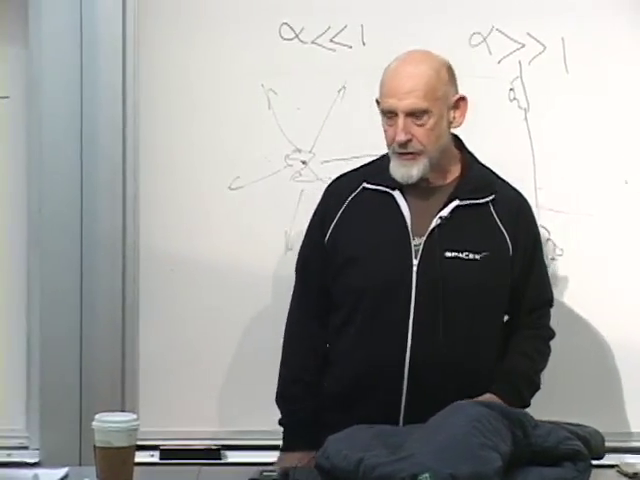
\includegraphics[width=0.72\textwidth]{lecture_01_figure_02.png}
\lectureframe{00:38:22.500}

\vspace{1em}

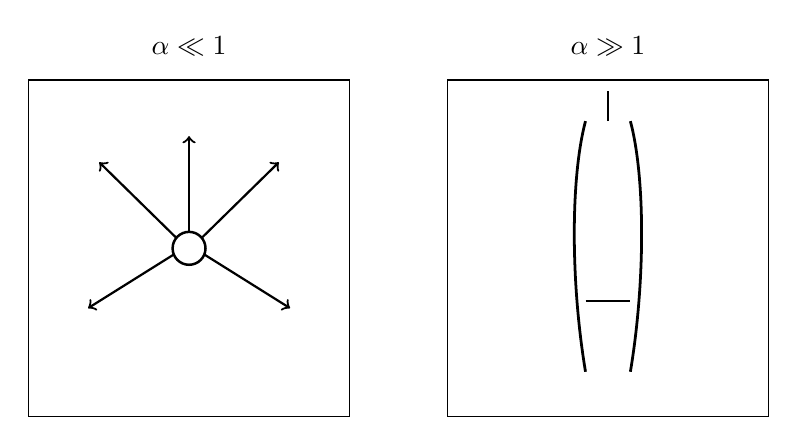
\begin{tikzpicture}[scale=0.95]
\draw (-5.3,-2.4) rectangle (-1.0,2.1);
\draw (0.3,-2.4) rectangle (4.6,2.1);

\node at (-3.15,2.55) {$\alpha \ll 1$};
\node at (2.45,2.55) {$\alpha \gg 1$};

\draw[line width=0.9pt] (-3.15,-0.15) circle (0.22);
\draw[->,line width=0.8pt] (-3.15,0.07) -- (-3.15,1.35);
\draw[->,line width=0.8pt] (-2.98,-0.01) -- (-1.95,1.00);
\draw[->,line width=0.8pt] (-3.32,-0.01) -- (-4.35,1.00);
\draw[->,line width=0.8pt] (-2.95,-0.23) -- (-1.80,-0.95);
\draw[->,line width=0.8pt] (-3.35,-0.23) -- (-4.50,-0.95);

\draw[line width=1.0pt] (2.15,-1.8) .. controls (1.95,-0.6) and (1.95,0.8) .. (2.15,1.55);
\draw[line width=1.0pt] (2.75,-1.8) .. controls (2.95,-0.6) and (2.95,0.8) .. (2.75,1.55);
\draw[line width=0.8pt] (2.15,-0.85) -- (2.75,-0.85);
\draw[line width=0.8pt] (2.45,1.55) -- (2.45,1.95);
\end{tikzpicture}
\caption{So sánh QED yếu--mạnh trong phần thảo luận về năng lượng tương tác. Hình vẽ tách riêng hai chế độ mà Susskind minh họa: một đám mây ghép yếu thưa loãng và một đám mây ghép mạnh tăng sinh.}
\end{figure}

Lý do hình này được đặt ở đây, dù phép so sánh yếu--mạnh đã được đưa ra trước đó, là vì trong bài giảng Susskind vẽ lại sự tương phản ấy ở thời điểm muộn hơn này do câu hỏi dẫn dắt, khi đang thảo luận về năng lượng tương tác và cấu trúc tăng sinh.

\section{Các lý thuyết brane chẵn và chiều không gian phụ xuất hiện}

Cho đến thời điểm này, bài giảng đã dựng nên một câu chuyện rất thuyết phục về sự hoán đổi: fermion so với boson, electron so với monopole, F-string so với D-string. Bước tiếp theo còn gây ngạc nhiên hơn. Susskind chuyển sang một phiên bản khác của lý thuyết dây, một phiên bản có các D-brane số chiều chẵn thay vì số chiều lẻ. Sự phân biệt này quan trọng vì trong lý thuyết đó không có D-string để hoán đổi với F-string. Ở đó có các D0-brane, D2-brane, D4-brane, v.v.

Vì thế, giới hạn ghép mạnh không thể đơn giản chỉ là việc đổi nhãn từ dây này sang dây khác. Theo bài giảng, có điều gì đó còn lạ hơn xảy ra: một chiều không gian phụ trở nên hiển lộ. Susskind cố ý phát biểu điều này trước hết dưới dạng kịch tính nhất --- ``một chiều mới xuất hiện'' --- rồi lập tức chuyển nó thành phát biểu cẩn trọng hơn: một chiều compact rất nhỏ nở ra cho đến khi không thể tiếp tục bỏ qua nữa.

Việc kiểm đếm này chính là một phần của ý chính, nên ông dừng lại ở đó:
\begin{equation}
\begin{aligned}
10\text{-dimensional string theory} &= 9\text{ space}+1\text{ time},\\
11\text{-dimensional theory} &= 10\text{ space}+1\text{ time}.
\end{aligned}
\end{equation}
Theo bài giảng, giới hạn ghép mạnh của lý thuyết brane chẵn về mặt hiệu dụng là mười một chiều.

\editorialnote{Lý thuyết brane chẵn là lý thuyết dây loại IIA, và sự hoàn chỉnh của nó trong miền liên kết mạnh là lý thuyết M. Trong các đơn vị chuẩn, bán kính của đường tròn xuất hiện và độ dài Planck mười một chiều tỉ lệ như \(R_{11}=g_s\ell_s\) và \(\ell_{11}=g_s^{1/3}\ell_s\). Những tên gọi và công thức này làm tường minh bảng đối chiếu hiện đại đứng sau cách trình bày hình học của bài giảng.}

\subsection{Bánh sandwich bơ đậu phộng}

Để hình dung chiều compact, Susskind dùng mô hình ``bánh sandwich bơ đậu phộng'': hai lát bánh mì mỏng vô hạn, với không gian thực ở giữa chúng. Quy tắc đặc biệt là đi ra ở một phía thì quay trở lại ở phía kia. Trong một ký hiệu thông thường mà bài giảng mô tả bằng hình ảnh hơn là bằng hình thức, ta có thể viết
\begin{equation}
y \sim y + 2\pi R.
\end{equation}
Nếu \(R\) rất nhỏ, những người quan sát sống trong chiếc sandwich đó sẽ mô tả thế giới của mình một cách hiệu dụng như có số chiều thấp hơn. Khi đó, cập nhật then chốt ở liên kết mạnh là
\begin{equation}
g\uparrow
\qquad \Longrightarrow \qquad
R_{\mathrm{compact}}\uparrow.
\end{equation}
Đó là điều Susskind muốn nói khi ông bảo rằng một chiều không gian mới xuất hiện: không phải không gian được tạo ra từ hư không, mà là một chiều compact vốn trước đây rất nhỏ nay nở ra và trở nên nhìn thấy được trong lý thuyết hiệu dụng.

\begin{figure}[htbp]
\centering
\resizebox{\linewidth}{!}{%
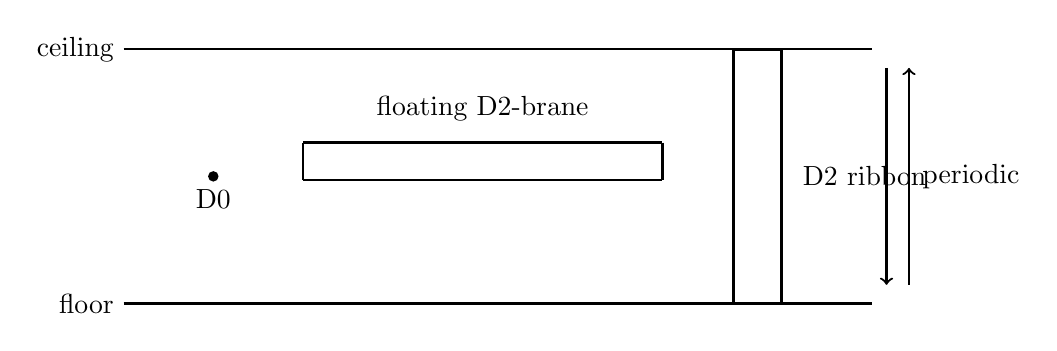
\begin{tikzpicture}[scale=0.95]
\draw[line width=0.9pt] (-5,1.7) -- (5,1.7);
\draw[line width=0.9pt] (-5,-1.7) -- (5,-1.7);

\node[left] at (-5,1.7) {ceiling};
\node[left] at (-5,-1.7) {floor};

\draw[->,line width=0.8pt] (5.2,1.45) -- (5.2,-1.45);
\draw[->,line width=0.8pt] (5.5,-1.45) -- (5.5,1.45);
\node[right] at (5.55,0) {periodic};

\draw[line width=1.0pt] (-2.6,0.45) -- (2.2,0.45);
\draw[line width=1.0pt] (-2.6,-0.05) -- (2.2,-0.05);
\draw[line width=1.0pt] (-2.6,0.45) -- (-2.6,-0.05);
\draw[line width=1.0pt] (2.2,0.45) -- (2.2,-0.05);
\node at (-0.2,0.9) {floating D2-brane};

\draw[line width=1.0pt] (3.15,-1.7) -- (3.8,-1.7);
\draw[line width=1.0pt] (3.15,1.7) -- (3.8,1.7);
\draw[line width=1.0pt] (3.15,-1.7) -- (3.15,1.7);
\draw[line width=1.0pt] (3.8,-1.7) -- (3.8,1.7);
\node[right] at (3.95,0) {D2 ribbon};

\fill (-3.8,0) circle (0.07);
\node[below] at (-3.8,-0.05) {D0};
\end{tikzpicture}
}%
\caption{Phép compact hóa kiểu sandwich. Biên trên và biên dưới được đồng nhất tuần hoàn; một D2-brane lơ lửng giữa chúng như một tấm thảm, còn một brane cùng loại khác kéo dài từ sàn lên trần và trông giống một dây khi chiều compact nhỏ.}
\end{figure}

\subsection{D0-brane và D2-brane sẽ ra sao?}

Bài giảng lúc này hỏi điều gì xảy ra với các D0-brane và các dây. Câu trả lời là bất đối xứng. Khi \(g\) trở nên lớn, các D0-brane ngày càng nhẹ đi; trong cách diễn giải cao chiều hơn, chúng gia nhập tháp các hạt mang xung lượng theo phương mới trở nên hiển hiện. Vì vậy, một đối tượng nặng nề, phức tạp trong mô tả liên kết yếu trở thành một kích thích nhẹ, thông thường trong mô tả liên kết mạnh.

Hệ thức khối lượng cho thấy sự đồng nhất sau đây:
\begin{equation}
M_{D0}(n)=\frac{n}{g_s\ell_s}
=\frac{n}{R_{11}}
=M_{\mathrm{KK}}(n).
\end{equation}
\editorialnote{Susskind gọi các D0-brane là ``các graviton'' của lý thuyết mười một chiều. Chính xác hơn, các trạng thái liên kết của chúng là các mode xung lượng Kaluza--Klein của bội siêu hấp dẫn mười một chiều, mà phần không khối lượng của nó chứa graviton. Sự phân biệt này giữ nguyên sự đồng nhất vật lý của bài giảng đồng thời tránh cách nói quá theo nghĩa đen như thể đó là một hạt đơn lẻ.}

Các D2-brane giải thích số phận của các dây. Có hai cấu hình được nhấn mạnh trong bài giảng:
\begin{enumerate}
\item một D2-brane lơ lửng giữa sàn và trần như một tấm thảm trong lớp bơ đậu phộng;
\item một D2-brane kéo dài từ sàn lên trần như một dải ruy băng, mở rộng theo phương nhìn thấy được.
\end{enumerate}
Khi chiếc sandwich mỏng, dải đó trông, về mặt hiệu dụng, như một đối tượng một chiều. Đó là đối tượng mà các quan sát viên năng lượng thấp gọi là một dây. Khi chiều compact mở ra, chính đối tượng ấy trở nên rõ ràng là giống màng. Vì giờ đây nó chứa nhiều vật chất hơn theo phương thẳng đứng, nó trở nên nặng và không còn giống dây nữa.

\paragraph{Lôgic của sự chuyển tiếp.}
\begin{enumerate}
\item Hãy bắt đầu với một chiều compact rất mảnh, để dải từ sàn tới trần ứng xử hiệu dụng như một sợi dây.
\item Tăng \(g\) lên, và chiều compact nở ra.
\item Các D0-brane trở nên nhẹ và được diễn giải lại như các trạng thái xung lượng Kaluza--Klein trong lý thuyết số chiều cao hơn.
\item Dải D2 giống dây trở thành một màng kéo dài thấy rõ và trở nên nặng.
\end{enumerate}
Đây là điểm bản lề của bài giảng khi chuyển từ đối ngẫu sang hình học xuất hiện. Liên kết mạnh không chỉ đơn thuần hoán đổi vật thể này lấy vật thể khác; nó thay đổi hình học nào mới là mô tả hữu hiệu.

Susskind dừng lại ở việc điều này nghe kỳ lạ đến mức nào. Mạng lưới các sự đồng nhất hóa được đề xuất đòi hỏi những quan hệ nhất quán toán học khó khăn, một số trong đó ban đầu xuất hiện trước các nhà vật lý như những phỏng đoán và về sau được các nhà toán học xác lập. Điều ông khẳng định không phải là mọi chân không dây thực tế đều đã được hiểu, mà là chính mạng lưới đối ngẫu ấy đã đứng vững qua những kiểm tra nghiêm ngặt khác thường.

Nếu hằng số liên kết biến thiên từ nơi này sang nơi khác trong thiết lập lý tưởng hóa này, thì mô tả hình học hữu hiệu cũng có thể biến thiên theo nó. Một vùng có thể trông gần như mười chiều, với các dây nhẹ và các D0-brane nặng; một vùng khác có thể mở ra thành mô tả mười một chiều, với các màng quấn nặng và các mode xung lượng Kaluza--Klein nhẹ. Sự thay đổi cục bộ của ngôn ngữ mô tả là một phần của cùng một mạng lưới đối ngẫu.

Bản ghi chép thoáng chốc chép tên của các quan hệ này thành ``các bất đẳng thức.'' Trong ngữ cảnh này, từ được nhắm tới là \emph{các đối ngẫu}: những quan hệ giữa các đầu đối nghịch của không gian tham số. Sự hiệu đính này quan trọng vì kết luận của bài giảng chính xác là không hề biết một danh sách duy nhất các thành phần cơ bản. Dây, brane, hạt và hình học nhiều chiều có thể biến đổi lẫn vào nhau; hoặc không thành viên nào của mạng lưới là tuyệt đối cơ bản, hoặc một sự tổ chức sâu hơn nào đó vẫn còn chưa biết.

\section{Các D3-brane, các màng quấn, và bức tranh hình học về đối ngẫu}

Sau giờ nghỉ, Susskind mô tả tường minh chủ đề này như một ``mạng lưới khổng lồ'' gồm các lý thuyết và ý tưởng liên kết với nhau. Các ví dụ tiếp theo không phải là những hiệu ứng cô lập mới; chúng là những cây cầu nối các ví dụ trước lại với nhau.

\subsection{Thể tích thế giới của một D3-brane}

Cây cầu đầu tiên sử dụng một D3-brane. Một D3-brane có ba chiều không gian, và một quan sát viên bị giới hạn trên nó có thể dễ dàng ngỡ đó là không gian thông thường. Brane có thể uốn cong và dao động, còn các dây kết thúc trên nó có thể nối lại, tách ra và tán xạ. Đối với một quan sát viên chỉ thấy các chiều dọc theo brane, mỗi đầu mút trông như một hạt và các tương tác giữa những đầu mút trông như một lý thuyết trường lượng tử thông thường.

\begin{figure}[htbp]
\centering
\resizebox{\linewidth}{!}{%
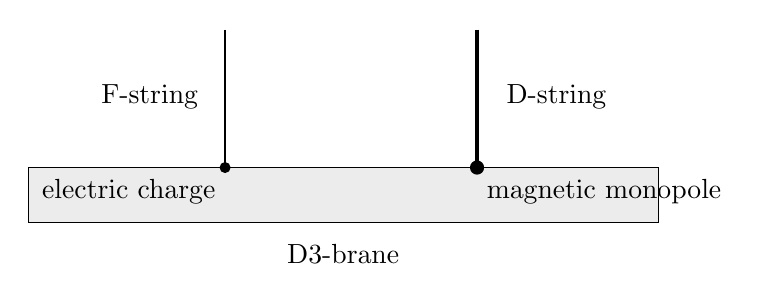
\begin{tikzpicture}[scale=1.0]
\draw[fill=gray!15] (-4,-0.35) rectangle (4,0.35);
\node at (0,-0.75) {D3-brane};

\draw[line width=0.9pt] (-1.5,2.1) -- (-1.5,0.35);
\fill (-1.5,0.35) circle (0.07);
\node[left] at (-1.72,1.25) {F-string};
\node[below left] at (-1.5,0.32) {electric charge};

\draw[line width=1.5pt] (1.7,2.1) -- (1.7,0.35);
\fill (1.7,0.35) circle (0.09);
\node[right] at (1.95,1.25) {D-string};
\node[below right] at (1.7,0.32) {magnetic monopole};
\end{tikzpicture}
}%
\caption{Diễn giải trên thể tích thế giới của D3-brane. Đầu mút của một F-string xuất hiện như một điện tích; đầu mút của một D-string xuất hiện như một đơn cực từ.}
\end{figure}

Đây là một trong những sự đồng nhất hóa thỏa đáng nhất của bài giảng. Một F-string kết thúc trên D3-brane xuất hiện đối với quan sát viên trên thể tích thế giới như một điện tích. Một D-string kết thúc trên cùng brane ấy xuất hiện như một đơn cực từ. Nói cách khác, đối ngẫu giữa F-string và D-string trở thành, trên thể tích thế giới của D3-brane, đối ngẫu điện--từ của lý thuyết trường thông thường. Điều trước đây là một phép tương tự nay đã trở thành một từ điển tường minh.

\editorialnote{Đối với một chồng các D3-brane, mô tả thể tích thế giới ở năng lượng thấp là lý thuyết Yang--Mills siêu đối xứng \(\mathcal N=4\) trong bốn chiều. Đối ngẫu điện--từ của nó là sự hiện thực hóa trong lý thuyết trường của đối ngẫu S của Type IIB; một brane đơn cho giới hạn Abel được dùng để minh họa bằng hình trong bài giảng.}

\subsection{Hai chiều compact và sự quấn bất đối xứng}

Sau đó Susskind quay trở lại hình học số chiều cao hơn và compact hóa không chỉ một mà hai chiều nhỏ. Vì không thể vẽ mười một chiều lên bảng, ông nén bảy chiều lớn không dùng trong hình phác thành một chiều ngang nhìn thấy được, rồi vẽ tường minh hai chiều compact. Ông nhấn mạnh phải vẽ phép compact hóa một cách bất đối xứng, vì một chiều compact phải ngắn hơn chiều kia nếu các dây hiệu dụng phải có lực căng khác nhau.

\begin{figure}[htbp]
\centering
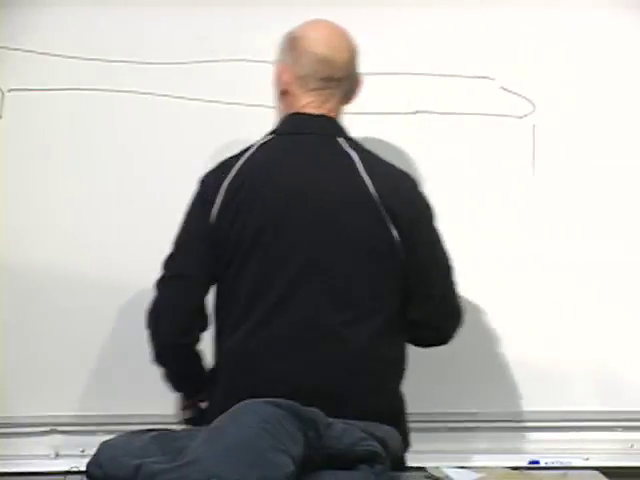
\includegraphics[width=0.78\textwidth]{lecture_01_figure_03.png}
\lectureframe{01:10:25.000}
\caption{Trạng thái hoàn chỉnh trên bảng của hai màng quấn. Chu trình compact ngắn và dài tạo ra các dải giống F-string và D-string được vẽ ở bên phải.}
\end{figure}

Một màng có thể quấn quanh một trong hai chiều compact và trông như một sợi dây khi nhìn từ các chiều không compact. Nếu \(R_1\) và \(R_2\) là hai bán kính vòng tròn, thì các lực căng hiệu dụng tương ứng của nó là
\begin{equation}
\begin{aligned}
T_{(1)}&=2\pi R_1 T_{\mathrm{M2}},\\
T_{(2)}&=2\pi R_2 T_{\mathrm{M2}},\\
\frac{T_{(1)}}{T_{(2)}}&=\frac{R_1}{R_2}.
\end{aligned}
\end{equation}
Do đó các kích thước vòng tròn không bằng nhau tạo ra các lực căng dây không bằng nhau. Nếu đồng nhất cách quấn theo chu trình ngắn hơn với F-string nhẹ và theo chu trình dài hơn với D-string nặng, ta có thể viết một cách sơ đồ
\begin{equation}
g_s\sim \frac{R_{\mathrm{short}}}{R_{\mathrm{long}}},
\qquad
\frac{T_{\mathrm{D1}}}{T_{\mathrm{F1}}}\sim \frac{1}{g_s}.
\end{equation}

\begin{classroomqa}
\audiencequestion{Liệu hằng số liên kết trong bức tranh này có thể được hiểu như tỉ số của hai chiều compact không? \lecturetimestamp{01:10:13}}
\lecturerresponse{Có. Tham số yếu--mạnh được hình học hóa thành một tỉ lệ cạnh. Làm cho một chiều ngắn đi tạo ra liên kết nhỏ; đổi chỗ hai chiều sẽ hoán đổi dây nhẹ và dây nặng.}
\end{classroomqa}

\editorialnote{Bài giảng tạm thời gọi tỉ số này là \(\alpha\), dùng lại ký hiệu trước đó đã dùng cho hằng số cấu trúc tinh tế của QED. Ở đây chúng tôi viết \(g_s\) để giữ cho hai nghĩa tách biệt nhau. Trong cấu trúc M-theory đầy đủ, hằng số liên kết Type IIB được mã hóa trong cấu trúc phức của xuyến compact hai chiều; tử số chính xác phụ thuộc vào cách các chu trình của nó được gán nhãn.}

Bức tranh màng quấn có thể được tóm tắt mà không cần đến phép méo phối cảnh của hình vẽ trên bảng:

\begin{figure}[htbp]
\centering
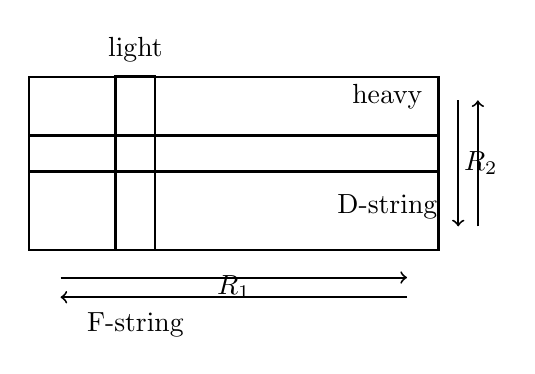
\begin{tikzpicture}[scale=1.0]
\draw[line width=0.9pt] (0,0) rectangle (5.2,2.2);
\node[below] at (2.6,-0.2) {\(R_1\)};
\node[right] at (5.4,1.1) {\(R_2\)};

\draw[->,line width=0.7pt] (5.45,1.9) -- (5.45,0.3);
\draw[->,line width=0.7pt] (5.7,0.3) -- (5.7,1.9);
\draw[->,line width=0.7pt] (0.4,-0.35) -- (4.8,-0.35);
\draw[->,line width=0.7pt] (4.8,-0.6) -- (0.4,-0.6);

\draw[line width=1.0pt] (1.1,0) -- (1.6,0) -- (1.6,2.2) -- (1.1,2.2) -- cycle;
\node at (1.35,2.55) {light};

\draw[line width=1.0pt] (0,1.45) -- (5.2,1.45);
\draw[line width=1.0pt] (0,1.00) -- (5.2,1.00);
\node at (4.55,1.95) {heavy};

\node at (1.35,-0.95) {F-string};
\node at (4.55,0.55) {D-string};
\end{tikzpicture}
\caption{Cả hai cấu hình màng quấn đều trông giống dây khi nhìn từ các chiều không compact, nhưng các thang compact không bằng nhau khiến một dây hiệu dụng nhẹ hơn dây kia.}
\end{figure}

Đây là phiên bản hình học của câu chuyện đối ngẫu trước đó. Thu ngắn một chiều trong khi kéo dài chiều kia làm một vật thể quấn nặng hơn và vật thể còn lại nhẹ hơn, vì thế vai trò của F-string và D-string có thể hoán đổi cho nhau.

\begin{classroomqa}
\audiencequestion{Nếu các chiều compact là tuần hoàn, các vật thể quấn có rộng vô hạn không? \lecturetimestamp{01:10:41}}
\lecturerresponse{Không. Một đường tròn compact có chu vi hữu hạn mặc dù ta có thể đi quanh nó lặp đi lặp lại mà không chạm tới mép. Phần trên và phần dưới của hình vẽ đã cắt mở biểu diễn cùng một điểm, cũng như hai đầu mút của một đoạn có thể biểu diễn một điểm của đường tròn.}
\end{classroomqa}

\begin{figure}[htbp]
\centering
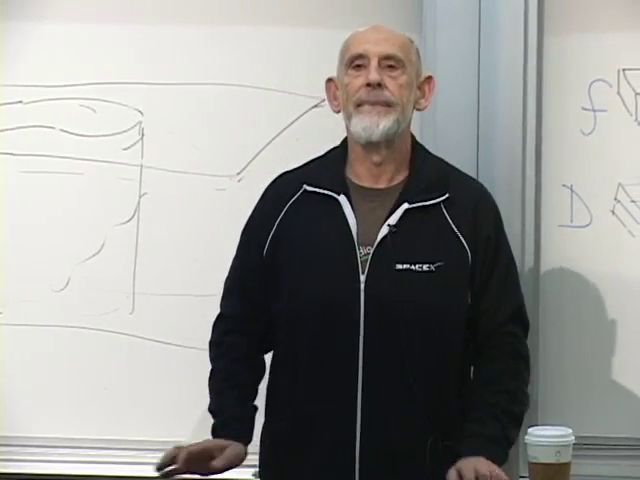
\includegraphics[width=0.78\textwidth]{lecture_01_figure_04.png}
\lectureframe{01:12:25.000}

\vspace{1em}

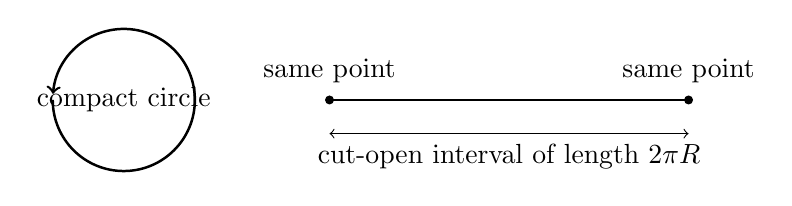
\begin{tikzpicture}[scale=0.95]
\draw[line width=0.9pt,->] (-3.7,0) arc[start angle=180,end angle=535,radius=0.95];
\node at (-2.75,0) {compact circle};
\draw[line width=0.9pt] (0.0,0) -- (4.8,0);
\fill (0.0,0) circle (0.06);
\fill (4.8,0) circle (0.06);
\draw[<->] (0.0,-0.45) -- (4.8,-0.45);
\node at (2.4,-0.75) {cut-open interval of length \(2\pi R\)};
\node[above] at (0.0,0.1) {same point};
\node[above] at (4.8,0.1) {same point};
\end{tikzpicture}
\caption{Một đường tròn compact và biểu diễn đã cắt mở của nó trên bảng. Đi qua một đầu mút sẽ trở lại ở đầu kia; còn đi quanh đường tròn đồng thời di chuyển theo một chiều không compact thì sẽ vạch ra một đường xoắn ốc.}
\end{figure}

\begin{classroomqa}
\audiencequestion{Tại sao đường đi theo chiều compact là một đường tròn chứ không phải một đường xoắn ốc? \lecturetimestamp{01:12:23}}
\lecturerresponse{Ở mỗi điểm cố định theo chiều không compact, chiều compact là một đường tròn. Chỉ khi ta tiến theo chiều không compact đồng thời quấn quanh đường tròn thì đường xoắn ốc mới xuất hiện. Đoạn trên bảng đơn giản chỉ là một đường tròn bị cắt mở, với hai đầu mút của nó được đồng nhất.}
\end{classroomqa}

\begin{classroomqa}
\audiencequestion{Liệu chính hình học này có giải thích được vì sao một D-brane có thể trông như một tập hợp các F-string khi bị thăm dò ở khoảng cách nhỏ không? \lecturetimestamp{01:12:49}}
\lecturerresponse{Mối liên hệ là có, nhưng nó không hiển nhiên trong bức tranh sơ cấp này; để thấy được điều đó cần thêm công cụ hình học. Hình vẽ nhằm tổ chức đối ngẫu, chứ không suy ra mọi mô tả thành phần vi mô.}
\end{classroomqa}

\begin{classroomqa}
\audiencequestion{Liệu chiều compact dài và ngắn có thể hoán đổi khi ta di chuyển trong không gian, hoặc khi thời gian tiến triển không? \lecturetimestamp{01:13:35}}
\lecturerresponse{Cả hai đều có thể trong mô hình lý tưởng hóa. Ép một chu trình lại trong khi làm nở chu trình kia sẽ hoán đổi dây quấn nào là nhẹ. Đây là một lý do nữa khiến ``dây cơ bản'' chỉ là một cái tên: mô tả được ưu tiên có thể thay đổi từ vùng này sang vùng khác hoặc theo thời gian.}
\end{classroomqa}

\section{Sự lý tưởng hóa, các điểm đối xứng đặc biệt và cảnh quan}

Phần cuối của bài giảng lùi ra khỏi những ví dụ đối ngẫu thanh nhã và hỏi xem chúng cho ta biết gì, và không cho ta biết gì, về thế giới thực.

Trước hết, Susskind cảnh báo rằng các đối ngẫu được kiểm soát chính xác là những đặc trưng của các lý thuyết siêu đối xứng đã được lý tưởng hóa cao độ, trong đó boson và fermion có khối lượng khớp nhau một cách chính xác. Phép tương tự của ông là các quỹ đạo tròn trong cơ học Newton: người ta nghiên cứu chúng trước tiên vì chúng đối xứng và dễ xử lý về toán học, chứ không phải vì chuyển động hành tinh thực tế được mô tả trọn vẹn bởi những đường tròn hoàn hảo. Hoàn toàn tương tự, các lý thuyết dây siêu đối xứng dễ phân tích hơn vì chúng đối xứng hơn mức mà tự nhiên dường như có.

Tuy vậy, sự lý tưởng hóa vẫn đem lại thông tin. Một quỹ đạo tròn hoàn hảo không phải là một hệ hành tinh thực tế, nhưng nó phô bày những đặc điểm còn tồn tại trong các quỹ đạo kém đối xứng hơn. Tương tự, các ví dụ siêu đối xứng cho thấy những cách nhất quán để cơ học lượng tử, hấp dẫn và cấu trúc vi mô có thể khớp với nhau. Cách phát biểu cố ý sắc gọn của Susskind là các lý thuyết dây có thể xử lý được không, theo nghĩa đen, phải là lý thuyết của thế giới chúng ta; giá trị của chúng nằm ở chỗ chúng bộc lộ những hiện tượng có khả năng xuất hiện trở lại trong những bối cảnh kém đối xứng hơn và khó xử lý hơn.

\subsection{Một bộ lắp ghép với nhiều kết quả}

D-brane chỉ là một phần của bộ lắp ghép sẵn có. Bài giảng cũng nhắc tới các thông lượng, orbifold và orientifold. Trước hết ta chọn một hình học compact, rồi chọn những brane và thông lượng nào chiếm các chu trình của nó. Ngay cả cấu hình sandwich đơn giản ấy cũng làm thay đổi vật lý số chiều thấp hơn khi ta chèn vào một D2-brane lơ lửng, hai cái, hoặc ba cái. Việc thêm hoặc bớt những thành phần như thế làm thay đổi các hạt, các tương tác và các tham số hiệu dụng.

Giả sử, theo phép đếm sơ đồ của bài giảng, một không gian compact sáu chiều có xấp xỉ \(500\) chu trình và mỗi chu trình chấp nhận cỡ \(10\) lựa chọn về brane quấn, thông lượng hoặc các cấu trúc liên quan. Khi đó số cách xây dựng tăng như
\begin{equation}
N_{\mathrm{vacua}} \sim 10^{500}.
\end{equation}
Lôgic đếm của bài giảng là sơ đẳng:
\begin{equation}
10 \times 10 \times \cdots \times 10 = 10^{500}
\end{equation}
với \(500\) thừa số. Phép tương tự với DNA nêu cùng ý đó trong một ngữ cảnh quen thuộc hơn:
\begin{equation}
N_{\mathrm{DNA}}(500)=4^{500}.
\end{equation}
Trong lúc so sánh với DNA, một người trong cử tọa kiểm tra rằng dọc theo một sợi có bốn khả năng: A, C, G và T. Sự đính chính ấy củng cố chứ không thay đổi lập luận. Một danh sách ngắn các lựa chọn cục bộ, được lặp lại nhiều lần, tạo ra một số lượng khổng lồ các cách sắp xếp toàn cục. Số mũ chính xác không phải là điều cốt yếu, và Susskind gọi \(10^{500}\) là một sự đánh giá thấp đã cũ; điểm mấu chốt là sự bùng nổ tổ hợp.

Điều này đem lại sự đảo ngược cuối cùng của kỳ vọng quy giản luận mở đầu. Vật lý hạt phức tạp không nhất thiết phải phát sinh từ các quy tắc vi mô phức tạp. Nó có thể phát sinh vì chân không của chúng ta là một cách sắp đặt phức tạp của nhiều thành phần đơn giản, cũng như một sinh vật phức tạp có thể được mã hóa bởi một chuỗi được xây từ bốn bazơ.

\begin{classroomqa}
\audiencequestion{Sau khi các mô tả tương đương có liên hệ với nhau bởi đối ngẫu đã được đồng nhất, liệu thông tin đầy đủ có chỉ chọn ra một hoặc vài chân không khả dĩ trong số này làm mô tả về thế giới của chúng ta không? \lecturetimestamp{01:26:11}}
\lecturerresponse{Có lẽ nó sẽ chọn ra một tập bị hạn chế, nhưng nhiều chân không phân biệt có thể trông cực kỳ giống nhau ở các năng lượng có thể tiếp cận. Con số cảnh quan được nêu ra được hiểu là vẫn còn lớn ngay cả sau khi các mô tả đối ngẫu đã được đồng nhất, và những chi tiết năng lượng cao không liên quan có thể hoạt động như ``DNA rác.''}
\end{classroomqa}

\subsection{Các điểm đối xứng và độ phức tạp điển hình}

Trong landscape có những điểm đối xứng đặc biệt. Trong bức tranh hình học, một cấu hình có tỷ lệ bằng nhau,
\begin{equation}
R_1=R_2,
\end{equation}
làm cho hai mô tả bằng dây quấn đơn giản ngang nhau. Trong phép tương tự điện--từ, điều này được biểu diễn một cách sơ đồ bởi
\begin{equation}
m_{\mathrm{monopole}}=m_e.
\end{equation}

\begin{figure}[htbp]
\centering
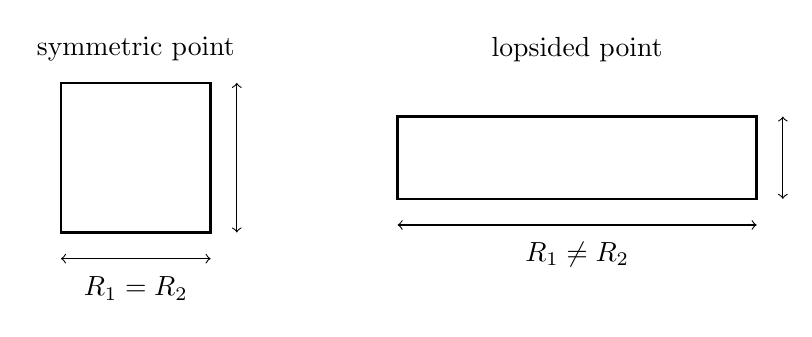
\begin{tikzpicture}[scale=0.95]
\draw[line width=0.9pt] (-4.5,-1.0) rectangle (-2.5,1.0);
\draw[<->] (-4.5,-1.35) -- (-2.5,-1.35);
\draw[<->] (-2.15,-1.0) -- (-2.15,1.0);
\node at (-3.5,1.45) {symmetric point};
\node at (-3.5,-1.75) {$R_1=R_2$};

\draw[line width=0.9pt] (0.0,-0.55) rectangle (4.8,0.55);
\draw[<->] (0.0,-0.9) -- (4.8,-0.9);
\draw[<->] (5.15,-0.55) -- (5.15,0.55);
\node at (2.4,1.45) {lopsided point};
\node at (2.4,-1.3) {$R_1\ne R_2$};
\end{tikzpicture}
\caption{Phép compact hóa có tỷ lệ bằng nhau đặt hai dây quấn vào vị thế đối xứng; phép compact hóa bất cân xứng làm cho một mô tả nhẹ hơn rất nhiều so với mô tả kia.}
\end{figure}

\begin{classroomqa}
\audiencequestion{Có những chân không nào trong landscape mà ở đó cách xây dựng trở nên đơn giản hơn nhiều vì các mô tả bằng F-string và D-string trùng nhau không? \lecturetimestamp{01:27:21}}
\lecturerresponse{Có, có những điểm đối xứng đặc biệt. Thế giới của chúng ta dường như không ở một điểm như vậy: hạt điện quen thuộc và một đơn cực từ không có khối lượng bằng nhau. Vì sao tự nhiên lại ở một điểm bất cân xứng như vậy thì chưa rõ.}
\end{classroomqa}

\editorialnote{Việc electron--đơn cực có khối lượng bằng nhau là một đặc trưng có tính sơ đồ của một mô hình tự đối ngẫu được bảo vệ thích hợp, chứ không phải dự đoán của QED thông thường không siêu đối xứng. Nó diễn đạt ý tưởng về điểm đối xứng của bài giảng, chứ không phải một khẳng định về electron quan sát được.}

Susskind sau đó nhắc lại một phép tương tự từ lý thuyết truyền thông. Các mã ngẫu nhiên có thể tốt một cách phi thường, trong khi các mã dễ mô tả và giải mã nhất lại có cấu trúc toán học bổ sung và trong lịch sử thường cho hiệu năng kém hơn. Về sau lý thuyết mã hóa đã tìm ra những cách xây dựng có cấu trúc rất hiệu quả, nhưng phép tương tự vẫn còn nguyên: bất cứ thứ gì có thể được gọi tên hoặc mô tả một cách gọn ghẽ đều nằm ở một góc rất đặc biệt, có độ phức tạp thấp, của toàn bộ không gian các khả thể. Tương tự như vậy, những chân không của lý thuyết dây dễ tính toán nhất có thể đơn giản một cách không điển hình.

Vì thế, những câu hỏi thích hợp có thể thay đổi. Thay vì đòi hỏi phép compact hóa chính xác đến từng chi tiết vi mô, ta có thể hỏi những đặc trưng nào là chung hoặc điển hình trong một tập hợp rộng. Susskind trình bày điều này như một vấn đề nghiên cứu, không phải một kết luận đã ngã ngũ, và bác bỏ các lập luận mang tính ý thức hệ thay cho tính toán.

\subsection{Các câu hỏi vũ trụ học}

\begin{classroomqa}
\audiencequestion{Một chiều compact có chu vi cực lớn có khác biệt được về mặt quan sát so với một chiều vô hạn không, và chúng ta có biết ba chiều không gian lớn của mình là vô hạn không? \lecturetimestamp{01:30:03}}
\lecturerresponse{Chúng ta không biết rằng chúng là vô hạn. Một 3-cầu kín có thể giãn nở mà vẫn compact. Các phép đo độ gần phẳng chỉ cho một cận dưới đối với bán kính độ cong, cũng như việc khảo sát một cánh đồng gần như phẳng có thể đặt cận dưới cho kích thước Trái Đất mà không chứng minh rằng bề mặt của nó là vô hạn. Chỉ khi phát hiện được độ cong hoặc một phép đồng nhất toàn cục thì mới xác định được thang độ hữu hạn ấy.}
\end{classroomqa}

\begin{classroomqa}
\audiencequestion{Nếu độ ghép có thể biến thiên theo không gian trong mô hình lý tưởng hóa, thì trong thế giới thực một sự biến thiên như vậy có thể xảy ra như thế nào? \lecturetimestamp{01:32:43}}
\lecturerresponse{Không phải theo kiểu biến thiên trơn, không bị hạn chế, đã dùng trong ví dụ đối xứng. Khả năng thực tế sẽ được bàn sau là sự biến thiên thông qua các chuyển tiếp rời rạc giữa những vùng có các quy luật hiệu dụng khác nhau. Việc những bước nhảy như thế có xảy ra hay không là một câu hỏi vũ trụ học.}
\end{classroomqa}

\editorialnote{Cần đọc câu trả lời này như phần báo trước của bài giảng về các chân không thông lượng và các chuyển tiếp miền, chứ không phải như một định lý tổng quát cấm mọi trường vô hướng biến thiên trơn. Các quan sát ràng buộc rất chặt các biến thiên của những độ ghép không thứ nguyên, còn các cơ chế ổn định hóa quyết định liệu trong một mô hình cho trước vẫn còn các moduli liên tục hay không.}

Bản ghi không lưu lại câu hỏi cuối cùng của cử tọa. Phần trả lời còn sót lại nói rằng hiện tượng được nêu ra có thể xảy ra đối với một số loại lỗ đen nhưng không xảy ra ở chân trời của một lỗ đen Schwarzschild thông thường, mà chân trời của nó xét cục bộ là một nơi bình thường đối với một quan sát viên rơi tự do. Vì không thể khôi phục câu hỏi ấy một cách đáng tin cậy, nên không quy cho cuộc trao đổi này một khẳng định cụ thể nào hơn.

\section{Từ những viên gạch đến một mạng lưới các mô tả}

Hy vọng rằng các tầng sâu hơn của vật lý tất phải đơn giản hơn đã tỏ ra mong manh. Trong boson hóa \(1+1\) chiều, cùng một lý thuyết có thể được tổ chức hoặc theo fermion hoặc theo boson, với fermion xuất hiện trở lại dưới dạng một kink. Trong điện động lực học lượng tử, ghép yếu và ghép mạnh hoán đổi vai trò mô tả của electron và đơn cực từ. Trong lý thuyết dây, F-string và D-string lặp lại cùng một khuôn mẫu ấy, còn trong lý thuyết các brane chẵn, ghép mạnh còn đi xa hơn nữa: một chiều compact nở ra, các D0-brane trở thành các trạng thái xung lượng Kaluza--Klein, và các dây hiệu dụng được diễn giải lại như các màng quấn trong một hình học số chiều cao hơn. Vì vậy, lý thuyết trường lượng tử hiện đại và lý thuyết dây không cung cấp một câu trả lời duy nhất và dứt khoát cho câu hỏi ``đâu là những viên gạch và đâu là những ngôi nhà?'' Chúng cung cấp một mạng lưới các mô tả, mỗi mô tả hữu hiệu trong miền riêng của nó, cùng với một landscape khổng lồ của các cách xây dựng khả dĩ mà kết quả điển hình là sự phức tạp chứ không phải sự đơn giản.
